\appendix
\section{Resoconto delle attività di verifica}
\subsection{Verifiche sui processi}

\subsubsection{Documentazione}

\subsubsubsection{Indice di Gulpease}

\begin{table}[H]
	\centering
	\renewcommand\tabularxcolumn[1]{>{\Centering}m{#1}}
	\begin{tabularx}{\textwidth}{| c | X |} 
	\hline
	\textbf{Documento} & \textbf{Valore}\\
	\hline
	Analisi dei Requisiti & 93 \\
    \hline
	Norme di Progetto & 81\\
	\hline
	Piano di Progetto & 68\\
	\hline
	Piano di Qualifica & 71\\
	\hline
    	\caption{Indice di Gulpease}
	\end{tabularx}
\end{table}

\subsubsection{Pianificazione}
\begin{figure}[H]
	\centering
	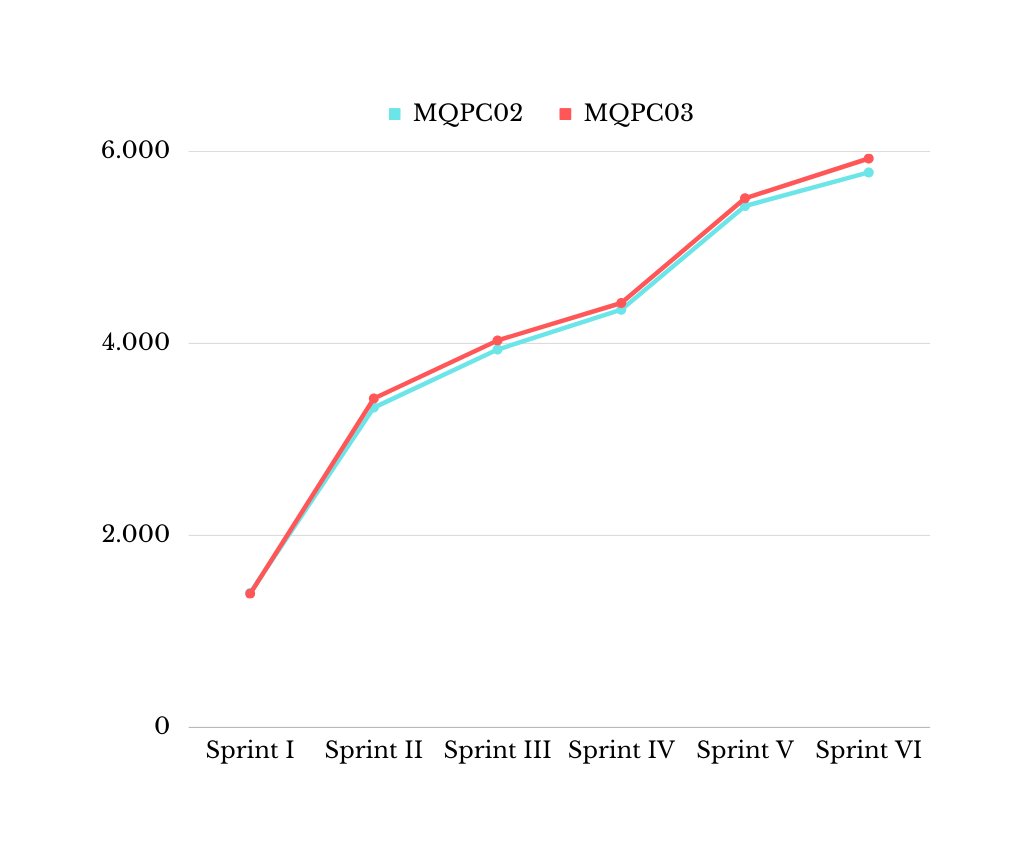
\includegraphics[scale=0.5]{img/BCWS-ACWS.png}
	\caption{Grafico che mostra l'andamento dei costi pianificati correlato a quelli reali}
\end{figure}
\begin{figure}[H]
	\centering
	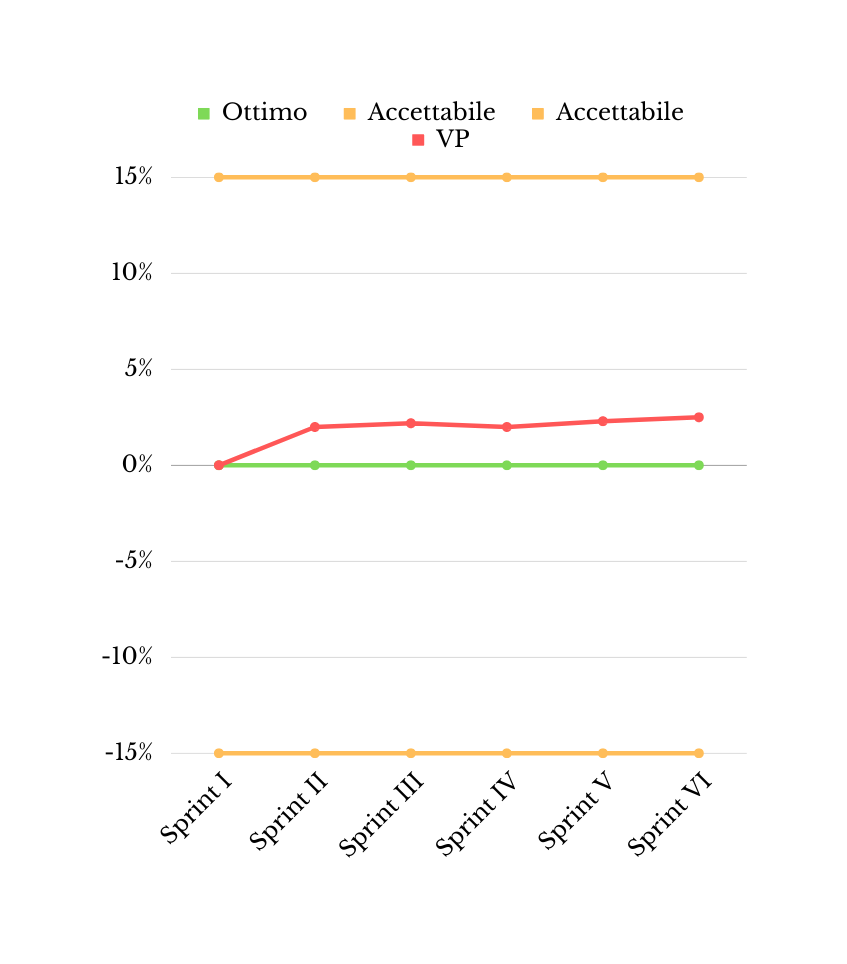
\includegraphics[scale=0.5]{img/SV.png}
	\caption{Grafico che mostra la differenza in percentuale tra le ore pianificate (ottime) e le ore effettivamente impiegate}
\end{figure}
\begin{figure}[H]
	\centering
	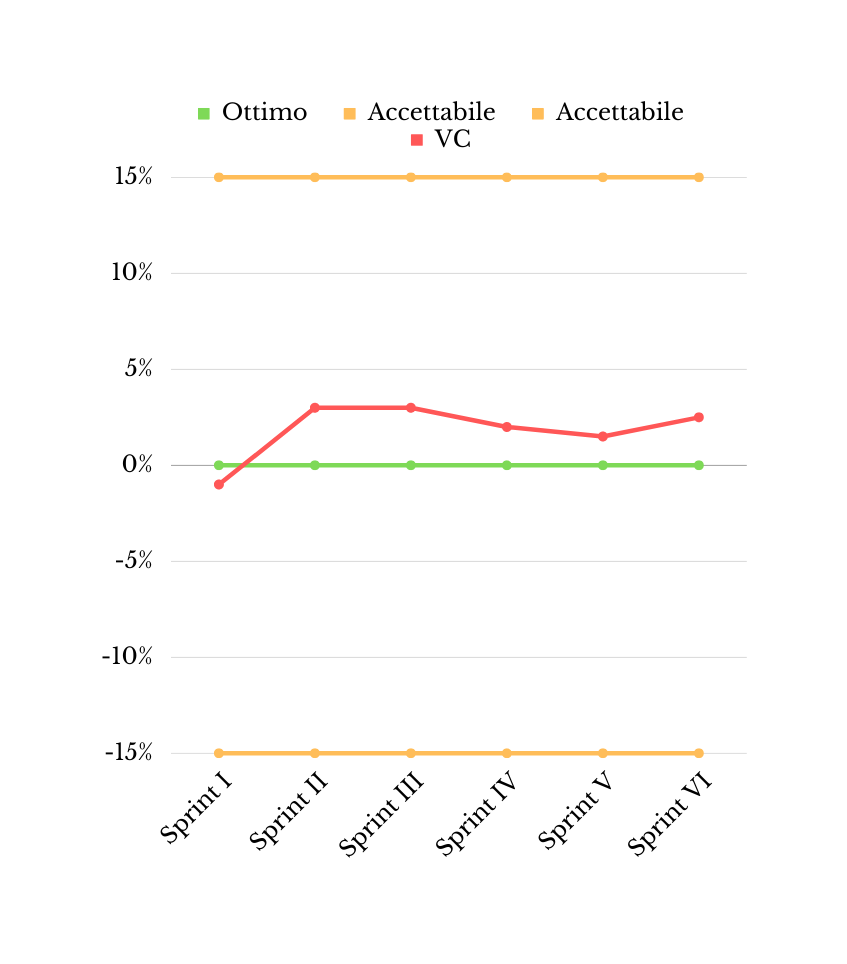
\includegraphics[scale=0.5]{img/CV.png}
	\caption{Grafico che mostra la differenza in percentuale tra i costi pianificati (ottimi) e i costi effettivi}
\end{figure}
